\documentclass[11pt]{article}
\usepackage[a4paper,margin=1in]{geometry}
\usepackage[T1]{fontenc}
\usepackage[utf8]{inputenc}
\usepackage{newtxtext,newtxmath}
\usepackage{amsmath,mathtools}
\usepackage{booktabs,tabularx}
\usepackage{graphicx}
\usepackage{microtype}
\usepackage{float}
\usepackage{hyperref}
\setlength{\emergencystretch}{3em}
\title{Supplementary Material\\Differentiable Ultrametric Routing for Hierarchical Evidence under Uncertain Provenance}
\author{K. A. Ulizko, A. S. Vatian, M. V. Ulizko, I. V. Tomilov, N. F. Gusarova}
\date{}
\begin{document}
\maketitle

This supplement retains technical and secondary material moved from the condensed submission manuscript. No result is introduced here that changes the interpretation of the main paper.

\section{Approximate ultrametric diagnostics}
Exact strong-triangle violations are discontinuous under arbitrarily small perturbations. For an approximate distance $\widehat d$, define
\begin{align}
V_0 &= \Pr\!\left[\widehat d_{xy}>\max(\widehat d_{xz},\widehat d_{yz})\right],\\
V_\varepsilon &= \Pr\!\left[
\frac{\widehat d_{xy}-\max(\widehat d_{xz},\widehat d_{yz})}
{\max(\widehat d_{xz},\widehat d_{yz})+\eta}>\varepsilon\right],\\
\Delta_{\rm ultra} &= \mathbb E\!\left[
\frac{\max\{0,\widehat d_{xy}-\max(\widehat d_{xz},\widehat d_{yz})\}}
{\max(\widehat d_{xz},\widehat d_{yz})+\eta}\right].
\end{align}
These diagnostics separate exact logical failure from numerically negligible reversals of the strong triangle inequality.

\section{Proof details for finite-depth routing}
\subsection{Hard-vertex exactness}
For one-hot passports, let the first mismatch occur at depth $k<D$. Then $P[d]=1$ for $d<k$ and $P[d]=0$ thereafter. The telescoping relaxation
\[
\widetilde d_{\rm tel}=\sum_{k=0}^{D-1}\rho^k(P[k-1]-P[k])
\]
has a single first-mismatch mass $\rho^k$. For the exponential relaxation, $\widetilde v=k$ and $P[D-1]=0$, giving $\widetilde d_{\rm exp}=\rho^k$. If all levels match, the telescoping sum is zero and the exponential form gives $\rho^D-\rho^D=0$. Hence both relaxations equal the finite prefix ultrametric at all hard vertices, including the zero diagonal.

\subsection{Full depth-sensitivity proof}
At the symmetric point $S[0]=\cdots=S[D-1]=s$, for every $d\geq m$,
\[
\frac{\partial P[d]}{\partial S[m]}=s^d.
\]
Differentiating the telescoping and exponential forms yields
\begin{align}
G_{\rm tel}(m)&=(1-\rho)\sum_{d=m}^{D-2}(\rho s)^d+(\rho s)^{D-1},\\
G_{\rm exp}(m)&=a_D\sum_{d=m}^{D-1}s^d+\rho^Ds^{D-1},
\end{align}
where
\[
v_D=s\frac{1-s^D}{1-s},\qquad a_D=(-\ln\rho)\rho^{v_D}.
\]
Consecutive differences satisfy
\begin{align}
G_{\rm tel}(m)-G_{\rm tel}(m+1)&=(1-\rho)(\rho s)^m>0,\\
G_{\rm exp}(m)-G_{\rm exp}(m+1)&=a_Ds^m>0,
\end{align}
so both profiles decrease strictly with depth. Because
\[
G_{\rm tel}(D-1)=(\rho s)^{D-1},\qquad
G_{\rm exp}(D-1)=s^{D-1}(a_D+\rho^D),
\]
direct substitution gives
\[
\frac{\kappa_{\rm tel}(D)}{\kappa_{\rm exp}(D)}
=\rho^{-(D-1)}C(\rho,s,D),
\qquad
C(\rho,s,D)=\frac{T_D(a_D+\rho^D)}{E_D},
\]
with $T_D=G_{\rm tel}(0)$ and $E_D=G_{\rm exp}(0)$.

To control $C$ uniformly in depth, set $L=-\ln\rho$ and
\[
a_- = L\rho s,\qquad a_+=\frac{L\rho s}{1-s},
\]
so that $a_-\leq a_D\leq a_+$. Also define
\[
t_-=1-\rho,\qquad t_+=\frac{1-\rho}{1-\rho s}+\rho s,
\]
and
\[
e_-=a_-,\qquad e_+=\frac{a_+}{1-s}+\rho^2s.
\]
Then $t_-\leq T_D\leq t_+$ and $e_-\leq E_D\leq e_+$ for all $D\geq2$, while $a_-\leq a_D+\rho^D\leq a_++\rho^2$. Therefore one may take
\[
c_1=\frac{t_-a_-}{e_+},\qquad
c_2=\frac{t_+(a_++\rho^2)}{e_-},
\]
which are positive, finite, and independent of $D$. For $\rho=1/p$, the explicit leading factor becomes $p^{D-1}$.

\subsection{Strictness and leakage proofs}
For hard pairs at common-prefix depths $k$ and $k+1$, shell similarities are $1-\rho^k$ and $1-\rho^{k+1}$. Multiplying their difference by the DSA structural scale $\gamma$ gives
\[
\Delta_k=\gamma(1-\rho)\rho^k,
\]
and maintaining a minimum structural separation $\tau$ through depth $k$ requires $\gamma\geq\tau/[(1-\rho)\rho^k]$.

For the leakage bound, choose any $b$ in the nearest shell $B$. For every visible $j\notin B$,
\[
z_{ij}-z_{ib}\leq2E_{\max}-\Delta_i.
\]
Since the softmax denominator is at least $\exp(z_{ib})$,
\[
A_{ij}\leq\exp(2E_{\max}-\Delta_i).
\]
Summing over $V_i\setminus B$ and clipping by the trivial bound one gives
\[
\sum_{j\in V_i\setminus B}A_{ij}
\leq \min\{1,|V_i\setminus B|\exp(2E_{\max}-\Delta_i)\},
\]
and rearrangement yields the sufficient condition
\[
\Delta_i\geq2E_{\max}+\log\frac{|V_i\setminus B|}{\varepsilon}
\]
for foreign-shell leakage at most $\varepsilon$.

\section{Secondary controlled-mechanism results}
\subsection{Exact-provenance visual summary}
Figure~\ref{fig:exact} is the visual counterpart of Table~1 in the main paper. It was removed from the main manuscript because the table already reports the exact numerical results.
\begin{figure}[H]
\centering
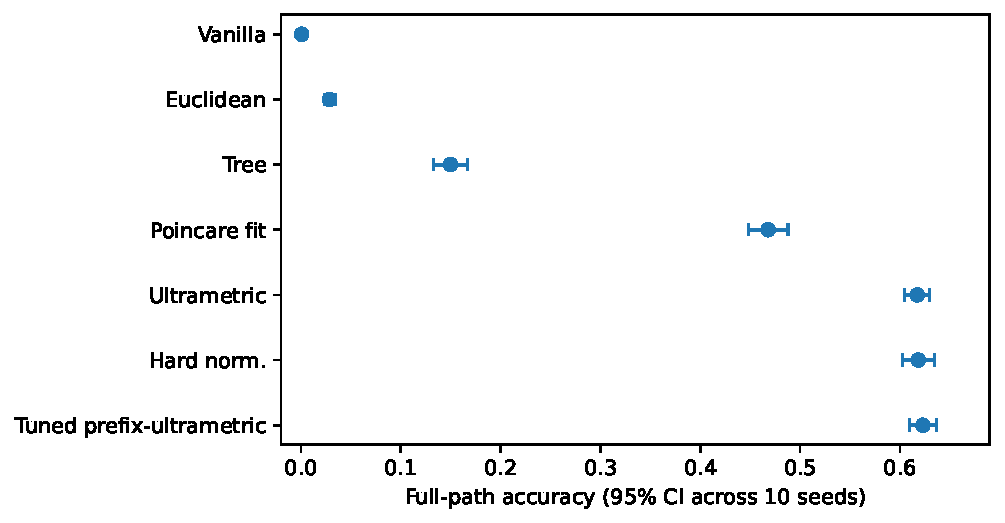
\includegraphics[width=.62\linewidth]{figures/fig_exact_provenance.pdf}
\caption{Ten-seed exact-provenance audit including the taxonomy-fitted hyperbolic baseline and hard/tuned-prefix-ultrametric controls.}
\label{fig:exact}
\end{figure}

\subsection{Soft-passport optimization detail}
Direct passport optimization separates the problem of learning a soft hierarchical address from the problem of consuming an already uncertain passport. Both relaxations recover all prefixes through depth eight. At depth 12, the telescoping form reaches 10 levels at the 90\% criterion while the exponential form reaches 12; for depths 16--96 they plateau near 10 and 14 levels. Conversely, shallow symmetric off-vertex smoothing can favor telescoping at fixed strictness. These results are consistent with the local cross-depth sensitivity theorem at its stated symmetric point; they are neither a task-level depth guarantee nor a claim of global optimization conditioning.

\subsection{Wrong-vote location intervention}
The same high-salience wrong vote placed in a foreign branch leaves structure-aware accuracy near clean levels, whereas placing it inside the admissible branch collapses provenance-only methods. Salience and semantic polarity are held fixed; only hierarchical provenance changes. The intervention therefore identifies provenance routing rather than contradiction semantics.
\begin{figure}[H]
\centering
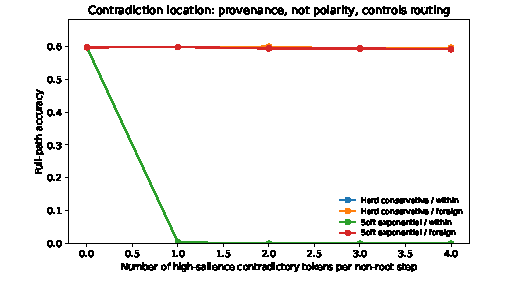
\includegraphics[width=.64\linewidth]{figures/fig_conflict_location.pdf}
\caption{Paired wrong-vote location intervention. Salience and wrong vote are fixed; only hierarchical provenance changes.}
\label{fig:wrongvote}
\end{figure}

\subsection{Secondary pretraining compatibility control}
A compact Transformer pretrained on an ontology-independent synthetic masked-token objective and then frozen preserves the structural ranking: fixed ultrametric readout reaches $0.805\pm0.027$ versus $0.670\pm0.029$ for tree distance over five seeds. This is a compatibility control rather than external-validity evidence; a randomly initialized frozen encoder already supports substantial structural routing. We therefore do not use this result to claim transfer to natural-language pretrained models.

\section{WOS metric definitions and additional paired statistics}
For a final leaf posterior $\pi$, gold leaf $c^*$, gold parent $b^*=g(c^*)$, and $\widehat c=\arg\max_c\pi_c$, define
\begin{align}
\operatorname{WrongParent}(\pi)&=\mathbf1\{g(\widehat c)\neq b^*\},\\
\operatorname{WrongBranchMass}(\pi)&=\sum_{c:g(c)\neq b^*}\pi_c
=1-\sum_{c:g(c)=b^*}\pi_c,\\
\operatorname{OutsideGold50}(\pi)&=\mathbf1\{\operatorname{WrongBranchMass}(\pi)>0.5\}.
\end{align}
The last quantity records whether aggregate posterior mass outside the gold parent exceeds 0.5. It does not imply that one wrong parent receives majority mass or that the argmax leaf lies outside the gold parent, and it is not a calibrated measure of application-level harm. NLL is $-\log\pi_{c^*}$ under the stated reporting floor; ECE uses 15 equal-width bins over $\max_c\pi_c$.

Table~\ref{tab:risk} reports the paired risk differences omitted from the condensed main manuscript. To keep interpretation metric-independent, every entry is expressed as improvement of ultrametric over the comparator: comparator risk minus ultrametric risk. Positive values therefore favor ultrametric for every row; the negative wrong-branch-mass value against Hard MAP reflects the concentration induced by exact support whenever the selected branch is correct.

\begin{table}[H]
\centering
\caption{Paired predicted-provenance improvements for principal risk-oriented metrics. Improvement is comparator risk minus ultrametric risk, so positive values favor ultrametric for every row; exact two-sided sign-flip tests use ten paired seeds.}
\label{tab:risk}
\scriptsize
\setlength{\tabcolsep}{4pt}
\begin{tabular}{lccc|ccc}
\toprule
& \multicolumn{3}{c}{Improvement vs Vanilla} & \multicolumn{3}{c}{Improvement vs Hard MAP}\\
Metric & $\Delta$ & 95\% CI & $p_{sf}$ & $\Delta$ & 95\% CI & $p_{sf}$\\
\midrule
NLL & $+.00213$ & $[+.00160,+.00266]$ & $.00195$ & $+5.63160$ & $[+5.59033,+5.67287]$ & $.00195$\\
Wrong-parent & $+.00515$ & $[+.00430,+.00600]$ & $.00195$ & $+.03696$ & $[+.03496,+.03896]$ & $.00195$\\
Wrong-branch mass & $+.01375$ & $[+.01354,+.01396]$ & $.00195$ & $-.03149$ & $[-.03328,-.02971]$ & $.00195$\\
Outside-gold $>.5$ & $+.00897$ & $[+.00830,+.00963]$ & $.00195$ & $+.01129$ & $[+.00898,+.01361]$ & $.00195$\\
\bottomrule
\end{tabular}
\end{table}

\section{Material retained in the reproducibility package}
The package records the exact ModernBERT model revision, embedding-extraction configuration, split definition, label-consistency audit, validation-selected routing parameters, all ten seed-level outputs, matched MAP-plus-finite-bias ablation, paired seed statistics, document-bootstrap outputs, theorem-verification results and executable verification code, and figure/table regeneration scripts. Candidate hyperparameter grids and full per-seed outputs remain machine-readable rather than duplicated in the manuscript.

\end{document}
